\section{QED $\beta$-function}
QED is an interacting quantum field theory, which has a dimensionless coupling between the photons and fermions. This means that interesting things can happen. Classically, the effect seems marginal, but we know that these statements do not survive quantum corrections. So, we study how these couplings flow under the renormalization group, which tells us the regime in which perturbation theory is valid.

Recall the QED path integral in the $R_\xi$ gauge:
\begin{equation}
    Z = \int \mathcal{D}A\mathcal{D}\psi \exp(i\int \bar{\psi}(i\slashed{D} - m)\psi - \frac{1}{4}F^2 - \frac{1}{2\xi}(\p_\mu A^\mu)) = \int \mathcal{D}A\mathcal{D}\psi e^{iS_0 + iS_{\text{int}}}
\end{equation}
with:
\begin{equation}
    D_\mu = \p_\mu + iA_\mu.
\end{equation}
The only non-Gaussian (and hence interaction) term in the action is:
\begin{equation}
    S_{\text{int}} = -e\int A_\mu \bar{\psi}\gamma^\mu \psi
\end{equation}

\subsection{Review of the Renormalization Group}
Last quarter, we saw how to do renormalization in the Wilsonian style, where we assume that some modes above some momentum $\Lambda$ have been already integrated out (removing any UV divergences), and then we perform an additional step of integrating out modes $b\Lambda < p < \Lambda$ (with $0 < 1 - b \ll 1$) and see how the couplings evolve under the process. This will tell us whether terms in the action will become more important or not.

\begin{center}
    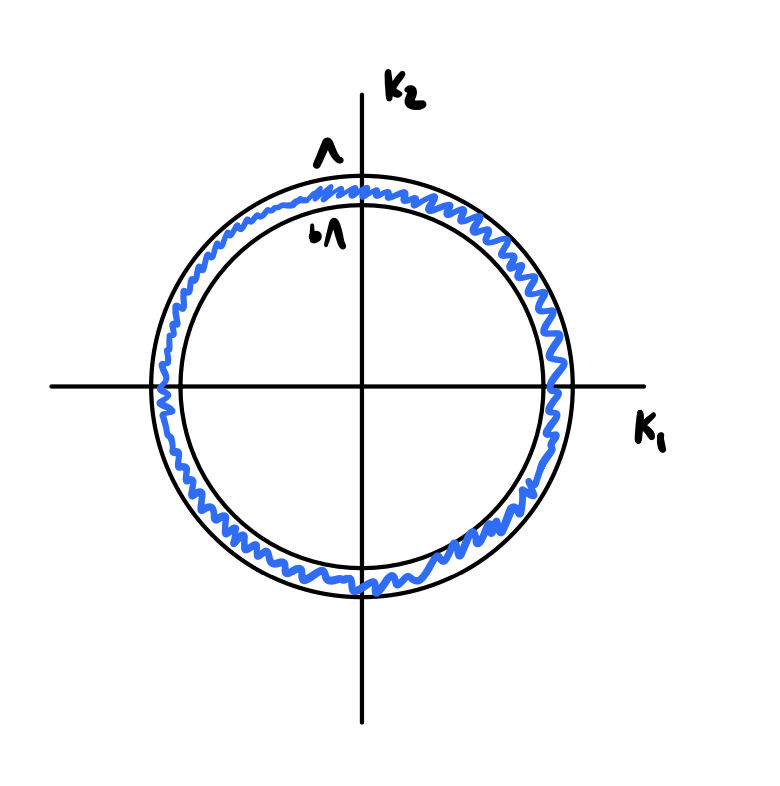
\includegraphics[scale=0.35]{Lectures/Images/lec11-energyshell.png}
\end{center}

Recall that in the scalar field case, we had:
\begin{equation}
    \phi(x) = \int_{p < \Lambda}e^{-ipx}\phi_p = \int_{p < b\Lambda}e^{-ipx}\phi_p + \int_{b\Lambda < p < \Lambda}e^{ipx}\phi_p = \phi_{b\Lambda} + \tilde{\phi}
\end{equation}
We then consider splitting the functional integral:
\begin{equation}
    \begin{split}
        Z &= \int \mathcal{D}\phi_\Lambda e^{iS[\phi]} 
        \\ &= \int \mathcal{D}\phi_{b\Lambda} e^{iS_0[\phi]}\int \mathcal{D}\tilde{\phi}e^{iS_0[\tilde{\phi}]}e^{iS_{\text{int}}[\phi, \tilde{\phi}]}
        \\ &= \int \mathcal{D}\phi_{b\Lambda} e^{iS_0[\phi]}\left(e^{i\delta S_{\text{eff}}[\phi]}\right)
        \\ &= \int \mathcal{D}\phi_{b\Lambda}e^{iS_{\text{eff}}[\phi]}
    \end{split}
\end{equation}
In the final step, we rescale coordinates such that:
\begin{equation}
    S_{\text{eff}} = \int d^4x \ldots = \int d^4\tilde{x} \ldots
\end{equation}
where:
\begin{equation}
    \tilde{x} = xb \implies \tilde{p} = \frac{p}{b} < \Lambda
\end{equation}
and canonically normalize.

\subsection{Applying RG to QED}
Before this final step, we expect the effective QED action will look like:
\begin{equation}
    S_{\text{eff}} = \int_x (1 + \delta_2)\bar{\psi}i\slashed{\p}\psi - (m + \delta m)\bar{\psi}\psi - (1 + \delta_1)eA_\mu \bar{\psi}\gamma^\mu \psi - \frac{1 + \delta_3}F^2 + \ldots
\end{equation}
where the $\ldots$ denotes irrelevant terms. We now rescale $x = \tilde{x}/b$ (and drop the $\tilde{}$s):
\begin{equation}
    S_{\text{eff}} = \int_x \frac{Z_2}{b^3}\bar{\psi}i\slashed{\p}\psi - \frac{m + \delta m}{b^4}\psi\bar{\psi} - \frac{Z_1e}{b^4}A_\mu \bar{\psi}\gamma^\mu \psi -\frac{Z_3}{4b^2}F^2 + \ldots
\end{equation}
We then canonically normalize:
\begin{equation}
    \psi \to \frac{b^{3/2}}{\sqrt{Z_2}}\psi, \quad A \to \frac{b}{\sqrt{Z_3}}A
\end{equation}
in order to normalize the kinetic terms. We then obtain:
\begin{equation}
    S_{\text{eff}} = \int_x \bar{\psi} i\slashed{\p}\psi  - \frac{m + \delta m}{bZ_2}\bar{\psi}\psi - \frac{Z_1 e}{Z_2\sqrt{Z_3}}A_\mu \bar{\psi}\gamma^\mu \psi - \frac{1}{4}F^2 + \ldots
\end{equation}
so we then have the new mass and coupling:
\begin{equation}
    \begin{split}
        m(b) &= \frac{m + \delta m}{bZ_2}
        \\ e(b) &= \frac{Z_1e}{Z_2\sqrt{Z_3}}
    \end{split}
\end{equation}
We can thus obtain the scale dependence of the couplings. Starting with $m$, which already has scale dependence at tree level ($Z \to 1, \delta m \to 0$):
\begin{equation}
    \beta_m \equiv \dod{m(b)}{\log b} = b\dod{m(b)}{b} = -m(b) < 0
\end{equation}
so $m$ is relevant (this was already clear from dimensional analysis). At lower and lower energies, mass matters more and more. The much more interesting thing to figure out is the scale dependence of $e$ - we already knew it was dimensionless from dimensional analysis, and this manifests in the $e(b)$ expression where there are no explicit factors of $b$ present. At tree level, $\beta_e = 0$ (marginal). Beyond tree level:
\begin{equation}
    \beta_e = \dod{}{\log b}\left(\frac{Z_1}{Z_2\sqrt{Z_3}}\right)e = e\dod{}{\log b}\frac{1 + \delta_1}{(1 + \delta_2)(1 + \delta_3)^{1/2}} \approx e\dod{}{\log b}\left(1 + \delta_1 - \delta_2 - \frac{1}{2}\delta_3\right)
\end{equation}

\subsection{Dimensional Regularization}
It is possible to study this with sharp cutoffs, but this breaks gauge invariance. So, it's not the best choice. A more convenient regulator in QED is is dimensional regularization - because dimension enters analytically in all of our formulas and loop integrals, we can analytically continue into $d = 4 - \e$. As you saw in your homework, $\log\Lambda$ divergences that come from dimensionless couplings with sharp cutoffs get replaced by $\frac{1}{\e}$ divergences ($\e \to 0$ to get back to 4 dimensions, so $\e^{-1}$ holds the UV divergences). More precisely, in RG, something like $\int \frac{d^4p}{p^4}$ becomes (with a sharp cutoff):
\begin{equation}
    \int_{b\Lambda}^\Lambda \frac{dp}{p} = \log\frac{\Lambda}{b\Lambda} = \log\frac{1}{b}
\end{equation}
vs. with dimensional regularization:
\begin{equation}
    \int_0^\infty \frac{dp}{p}p^{-\e} = \left.-\frac{1}{\e}p^{-\e}\right|_\mu^\infty = \frac{1}{\e}\mu^{-\e} = \frac{1}{\e}e^{-\e\log \mu} \approx \frac{1}{\e}(1 - \e\log\mu + \ldots) = \frac{1}{\e} - \log \mu
\end{equation}
so in the RG setting $\log\frac{1}{b}$s get replaced with $\frac{1}{\e}$s. As an example, we perform the following Feynman integral via the sharp cutoff method:
\begin{equation}
    \int_{b\Lambda}^\Lambda \frac{pdp}{p^2 + \Delta} = \left.\frac{1}{2}\log(p^2 + \Delta)\right|_{b\Lambda}^\Lambda = \frac{1}{2}\log\frac{\Lambda^2 + \Delta}{(b\Lambda)^2 + \Delta} \approx \log(\frac{1}{b}) + C\log\Delta + \ldots
\end{equation}
and via the dim reg method:
\begin{equation}
    \int_0^\infty \frac{p^{1-\e}dp}{p^2 + \Delta} = \frac{\pi}{2}\frac{1}{\sin(\frac{\e\pi}{2})}\Delta^{-\frac{\e}{2}} \approx \frac{1}{\e + O(\e^3)}\left(1 - \frac{\e}{2}\log\Delta + \ldots\right) = \frac{1}{\e} - \frac{1}{2}\log \Delta + \ldots
\end{equation}
The dim reg method provides the same results, but does allow us to compute things without breaking gauge invariance.

\subsection{Renormalizing the QED Coupling}
We start by computing $Z_3$, which corresponds to the renormalization of the photon propagator. You already did this in your homework, and we will see that $Z_1 = Z_2$ via a Ward identity, so this actually is the most important part. The diagram of interest is the one loop ($\avg{j^\mu j^\nu}$) diagram:

\begin{center}
    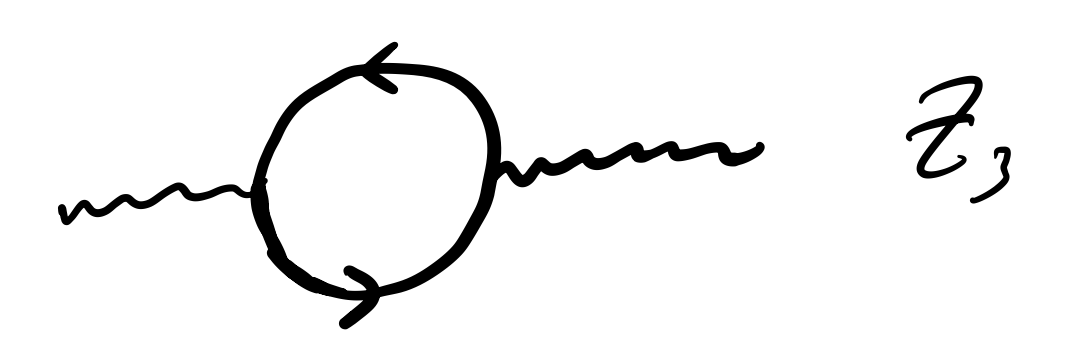
\includegraphics[scale=0.35]{Lectures/Images/lec11-Z3.png}
\end{center}

We have:
\begin{equation}
    S_{\text{int}}[\tilde{\phi}, \phi] \supset -e A_\mu \tilde{\bar{\psi}}\gamma^\mu \tilde{\psi}
\end{equation}
as the fermions get integrated out, so:
\begin{equation}
    Z = \int \mathcal{D}\phi e^{iS_0[\phi]}\int \mathcal{D}\tilde{\phi}e^{iS_{\text{int}}[\phi, \tilde{\phi}]}e^{iS_0[\tilde{\phi}]}
\end{equation}
expanding out the interacting action as a power series, the first contributing term is:
\begin{equation}
    \frac{i^2}{2}S_{\text{int}}^2 = -\frac{e^2}{2}\int_{x_1}A_\mu \tilde{\bar{\psi}}\gamma^\mu \tilde{\psi}\int_{x_2}A_\nu \tilde{\bar{\psi}}\gamma^\nu \tilde{\psi}
\end{equation}
So:
\begin{equation}
    \begin{split}
        \int \mathcal{D}\tilde{\phi}\frac{i^2}{2}S_{\text{int}}^2e^{iS_0[\tilde{\phi}]} &= -\frac{1}{2}e^2\int_1\int_2 A_\mu(x_1)A_\nu(x_2)\avg{j^\mu(x_1)j^\nu(x_2)}
        \\ &= -\frac{e^2}{2}\int \frac{d^4p}{(2\pi)^4}A_\mu(p)A_\nu(-p)\avg{j^\mu j^\nu}(p)
        \\ &= i\delta S_{\text{eff}}[\psi, A]
    \end{split}
\end{equation}
In your homework, you found that the current two point function was:
\begin{equation}
    \avg{j^\mu j^\nu}(p) = (p^2\eta^{\mu\nu} - p^\mu p^\nu)\frac{i}{6\pi^2}\frac{1}{\e}
\end{equation}
Therefore:
\begin{equation}
    S_{\text{eff}} = -\frac{e^2}{6\pi^2}\frac{1}{\e}\frac{1}{2}\int\frac{d^4p}{(2\pi)^4}A_\mu(-p)A_\nu(p)(p^2\eta^{\mu\nu} - p^\mu p^\nu)
\end{equation}
This looks identical to the Maxwell term:
\begin{equation}
    S_0 \supset -\frac{1}{2}\int_p A^\mu_p A^\nu_p(p^2 \eta^{\mu\nu} - p^\mu p^\nu)
\end{equation}
which is perhaps not surprising; we have a gauge invariant regulator, so we should get a gauge invariant result. We could have generated other gauge invariant terms, but these would contain higher derivatives; we focus on the terms that have a chance of being relevant. From this, we can identify the renormalization term $Z_3$:
\begin{equation}
    S_{\text{eff}} -\frac{1}{4}\left(1 + \frac{e^2}{6\pi^2}\frac{1}{\e}\right)\int_x F^2
\end{equation}
\begin{equation}
    Z_3 = 1 + \frac{e^2}{6\pi^2}\frac{1}{\e} \to 1 - \frac{e^2}{6\pi^2}\log(b)
\end{equation}
So we have the key ingredient in:
\begin{equation}
    \beta_e = \dod{}{\log b}\frac{Z_1}{Z_2\sqrt{Z_3}}e.
\end{equation}
We still need to calculate $Z_1, Z_2$. 

\begin{center}
    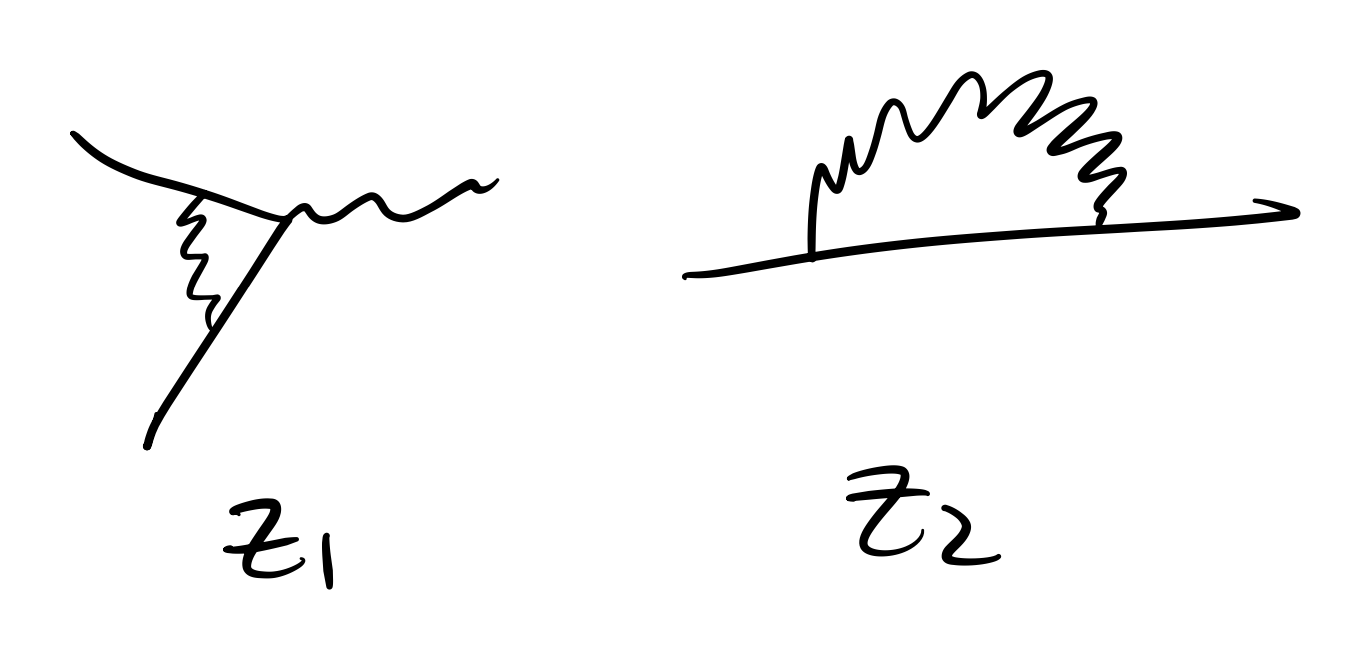
\includegraphics[scale=0.35]{Lectures/Images/lec11-Z1Z2.png}
\end{center}

But the ward identity implies they are equal (this will be the last thing we do this lecture). Thus the ratio drops out, and we end up with:
\begin{equation}
    \beta_e = \dod{}{\log b}\frac{e}{\sqrt{Z_3}} = e\dod{}{\log b}(1 - \frac{1}{2}\delta_3) = -\frac{e}{2}\dod{\delta_3}{\log b} = \frac{e^3}{12\pi^2} > 0
\end{equation}
Thus! $\beta_e > 0$ and so the coupling is \emph{irrelevant} under RG. Therefore, the interactions shrink at lower and lower energies. This also makes sense that it was one of the first QFTs to be discovered; we have access to low energies, and this is a regime where perturbation theory is controlled.

Conversely, interactions grow at higher energies, which tells us that QED is \emph{not} UV complete. In nature, this is UV-completed by the theory of non-abelian gauge fields.

\subsection{Last Step - Ward Identity}
We go through the argument of the Ward identity implying $Z_1 = Z_2$. We had shown that a consequence of the Ward identity was:
\begin{equation}
    i\p_\mu \avg{j^\mu_p \psi \bar{\psi}_{p'}} = G(p') - G(p+p')
\end{equation}
and in the amputated case:
\begin{equation}
    i\p_\mu \avg{j^\mu_p \psi \bar{\psi}_{p'}}_{\text{amp}} = \frac{1}{G(p + p')} - \frac{1}{G(p')}
\end{equation}
Where in the free theory:
\begin{equation}
    ip_\mu \gamma^\mu = i\slashed{p} \stackrel{?}{=} \frac{\slashed{p} + \slashed{p}' + m}{-i} - \frac{\slashed{p}' + m}{-i} = i\slashed{p}
\end{equation}
In the interacting theory, the vertex gets renormalized,so the LHS becomes:
\begin{equation}
    \gamma^\mu Z_1 = \avg{j^\mu \psi\bar{\psi}}_{\text{amp}}
\end{equation}
and the fermion propagator gets normalized:
\begin{equation}
    S_{\text{eff}} \supset \int Z_2\bar{\psi}i\slashed{\p}\psi \implies G(p) = \frac{-i}{Z_2\slashed{p} + (m + \delta m)}
\end{equation}
so the RHS becomes:
\begin{equation}
    Z_2i\slashed{p}
\end{equation}
This implies:
\begin{equation}
    i\slashed{p} Z_2 = i\slashed{p}Z_2 \implies Z_1 = Z_2.
\end{equation}
This is not at all obvious from looking at the Feynman diagrams leading to these two terms; they look different and the 1-loop calculations are tedious. Such is the power of symmetry!

Thus, we've deduced the fate of QED. Next, we will slightly switch gears, and study scattering in QED (where the setting is richer, e.g. due to particles having spin). Further, there is a subtlety when looking at scattering of massless particles - the existence of a mass gap was crucial for well-separating the single-particle excitations from the two-particle continuum. We don't have this in QED due to the photons being gapless. So the S-matrix of QED does not formally exist. So what have people been doing for the last century? It is possible to work out these subtleties, which we will go through. The fundamental problem is we can't distinguish whether we have a particle or $n$ super low energy photons. Naively we get IR divergences (large wavelength phenomena) which gets out of control. We'll see how to control it, next.